% GMC-Link — ACM Multimedia Asia 2026 Regular Paper
% Double-blind submission: sigconf + review + anonymous.
% Build: latexmk -pdf main.tex   (acmart.cls from system TeX Live)
\documentclass[sigconf,anonymous,nonacm]{acmart}

\usepackage{multirow}              % per-host recipe table
\usepackage{microtype}             % kills sub-3pt overfull, polishes justification
\usepackage{tikz}                  % Fig 1 pipeline + Fig 2 ego-motion schematic (self-contained, no asset)
\usetikzlibrary{arrows.meta,positioning,fit,backgrounds}
\captionsetup{textfont={normalfont}}  % bold label, normal description (lead-in phrases bolded per caption)
\settopmatter{printacmref=false}   % no ACM ref block in review draft
\setcopyright{none}
\acmConference[MM Asia '26]{ACM International Conference on Multimedia in Asia}{December 2026}{Location TBD}
\acmYear{2026}
\settopmatter{printfolios=false}    % pure paper copy without reviewer page numbers
\renewcommand\footnotetextcopyrightpermission[1]{} % remove ACM conference/copyright footer
\emergencystretch=1em

\begin{document}

\title{Recovering Motion-Referring Expressions in Moving-Camera Videos via Global Motion Compensation}

\author{Anonymous Author(s)}
\affiliation{%
  \institution{Submission under double-blind review}
  \country{}
}

\begin{abstract}
  Referring multi-object tracking (RMOT) takes a video and a natural-language expression as input and tracks all objects described by the expression. Many expressions describe how an object moves rather than how it appears, yet existing RMOT models often infer motion from raw bounding-box displacement. Under a moving camera, this signal is unreliable: a parked vehicle may appear to move across the image, while a vehicle moving with the camera may show little displacement on the image and be incorrectly treated as static. Existing motion-language RMOT methods align motion with text but do not explicitly remove camera-induced motion, whereas ego-motion compensation in multi-object tracking stays inside the tracker, stabilizing track states for association, and never reaches the language-matching stage. We bridge these two directions with Global Motion Compensation-Link (GMC-Link), a decision-level plug-in with host-specific score calibration. GMC-Link composes frame-to-frame homographies into a cumulative transform, extracts residual motion at multiple temporal gaps, compares the resulting motion feature with the language expression using separate motion and text encoders, and adds the resulting motion-matching score to the host prediction without retraining the host model. On iKUN~\cite{ikun}, GMC-Link improves moving-class Higher Order Tracking Accuracy (HOTA)~\cite{hota} from $20.25$ to $29.08$, corresponding to a gain of $8.83$ points over five random seeds. Most of this improvement comes from introducing motion-language alignment, while ego-motion compensation provides a further gain of $1.77$ moving-class HOTA ($p{=}0.006$) and $2.07$ static-class HOTA ($p{<}10^{-4}$) over raw image-plane motion. These results show that compensation helps both recover truly moving objects and reject stationary objects affected by camera motion. Across the three evaluated host--split settings, larger gains are observed for hosts with lower native moving-class HOTA. In pooled HOTA, GMC-Link matches the published iKUN result and improves FlexHook~\cite{flexhook} on Refer-KITTI V2~\cite{temprmot} by $0.281$, while FlexHook on Refer-KITTI V1~\cite{transrmot} remains below its published score because of a known reproduction gap.
\end{abstract}

\keywords{referring multi-object tracking, ego-motion compensation, motion-language alignment, plug-in module, Refer-KITTI, video grounding}

\maketitle
\thispagestyle{empty}
\pagestyle{empty}

\section{Introduction}
\label{sec:intro}

Referring multi-object tracking (RMOT) outputs trajectories for the objects described by a free-form language. For example, a language description such as \emph{"left-vehicles-in-red"} in the Refer-KITTI dataset is used to evaluate RMOT performance. Many of the descriptions in the Refer-KITTI dataset focus on object motion, such as ``moving cars'' or ``a vehicle turning left'', rather than appearance. However, in videos captured by a moving camera, the observed motion is a mixture of object motion and camera motion. As a result, a stationary car may appear to move because of camera motion, while a moving car may appear stationary if it moves together with the camera.

RMOT methods~\cite{transrmot,ikun,flexhook} match language against tracked objects, and recent work such as VMRMOT~\cite{vmrmot} adds explicit motion cues such as direction and speed change to that matching. All of these methods, however, compute motion from bounding-box displacement in the image, which under a moving camera mixes object motion with camera motion.

Conventional multi-object tracking (MOT) already removes camera motion: BoT-SORT~\cite{botsort} estimates camera-induced image motion, while UCMCTrack~\cite{ucmctrack} stabilizes object trajectories. However, the compensated motion never reaches the language-matching stage. We estimate camera motion directly from image features rather than from the global positioning system (GPS) and inertial measurement unit (IMU) streams provided by KITTI, so the module can be attached to different two-stage RMOT frameworks without modifying their architectures.

GMC-Link separates camera motion from object motion to provide motion information for language-guided tracking. It consists of four stages. First, a homography, which describes the geometric transformation between consecutive frames, is estimated to measure camera motion. The estimated homographies are accumulated over multiple frames to compensate for camera motion and provide a stable reference for measuring object motion. Second, residual velocity, which represents object motion after camera motion has been removed, is computed over multiple frames and used as a temporal motion feature. Third, the Contrastive Motion Aligner compares the motion feature with the language expression and produces a motion matching score. Finally, the motion score is combined with the host model through a calibrated decision-level correction, allowing GMC-Link to improve existing two-stage RMOT frameworks without modifying their architectures.

The accumulated homographies are the key component of GMC-Link. By compensating for camera motion, they allow the motion feature to represent the object's movement rather than the camera's movement. They also preserve motion information across multiple frames, enabling the model to capture motion patterns described by expressions such as ``moving'' or ``turning''. This design leads to a two-sided prediction that can be tested directly: if residual velocity is replaced with raw image velocity, moving-class accuracy should decrease because objects travelling with the camera lose their image displacement, and static-class accuracy should also decrease because parked objects inherit the camera's motion. Section~\ref{sec:exp} confirms both effects and shows that, among the module's design choices, camera motion compensation is the only one whose removal significantly degrades either class. Compensation therefore makes the motion feature effective for object disambiguation rather than simply providing additional motion cues.

This work connects ego-motion compensation with motion-language modeling for RMOT. Our main contributions are as follows.
\begin{itemize}
  \item We propose GMC-Link, a decision-level plug-in that aligns ego-compensated residual velocity with the referring expression and corrects the host score without modifying or retraining the host RMOT model.
  \item We show that among the module's design choices, camera motion compensation is the key factor: it is the only component whose removal significantly degrades both moving-class ($p{=}0.006$) and static-class ($p{<}10^{-4}$) HOTA.
  \item On iKUN, GMC-Link raises moving-class HOTA by $8.83$ while preserving the host's detector, tracker, and appearance-language matching, with positive gains on all three host--split settings and the largest gain on the host with the weakest native motion understanding.
\end{itemize}

\section{Related Work}
\label{sec:related}

\subsection{Referring MOT and motion-language fusion}
TransRMOT~\cite{transrmot} introduced the RMOT task on Refer-KITTI. Later methods improved different parts of this task. For example, iKUN~\cite{ikun} separated language-based object matching from object tracking, while FlexHook~\cite{flexhook} improved how visual and language information interact. ReferGPT~\cite{refergpt} uses a multimodal large language model to describe existing object tracks, and MEX~\cite{mex} provides a memory-efficient module for matching tracks with language.

More recent RMOT methods~\cite{mlstrack,deeprmot,cdrmot,tellmewhat} further improve how models understand object descriptions. VMRMOT~\cite{vmrmot}, for example, explicitly represents motion using information such as position, direction, changes in distance, and changes in speed. However, these methods still estimate object motion from bounding-box movements in the image. When the camera moves, the observed bounding-box movement contains both the object’s own motion and the camera’s motion. Therefore, a stationary object may appear to be moving, while a moving object may appear nearly stationary. This makes it difficult for the model to correctly understand motion-related expressions.

TempRMOT~\cite{temprmot} is different because it already stores trajectory history in recurrent memory. In our experiments, adding our external motion module to TempRMOT reduced pooled Higher Order Tracking Accuracy (HOTA) in two separate trials. This result suggests that the additional module may introduce redundant motion information or unnecessary constraints because TempRMOT already models motion over time. We therefore focus on two-stage RMOT models that do not already encode trajectory history in recurrent memory.

\subsection{Camera and ego-motion compensation in tracking}

Camera motion compensation is widely used in traditional multi-object tracking (MOT) to improve tracking when the camera itself is moving. BoT-SORT~\cite{botsort} estimates camera-induced image motion between consecutive frames using Oriented FAST and Rotated BRIEF (ORB) feature matches~\cite{orb} and Random Sample Consensus (RANSAC)~\cite{ransac}. UCMCTrack~\cite{ucmctrack} instead estimates how the camera moves relative to the road surface. EMAP~\cite{emap} further separates the camera's turning and movement from object motion within the Kalman prediction process, improving HOTA on KITTI by more than $5\%$ across four trackers.

These methods demonstrate that compensating for camera motion can improve matching the same objects across frames. However, the compensated positions are mainly used to match objects between adjacent frames. They are not accumulated over time to describe an object's motion, nor are they connected to language expressions such as ``moving,'' ``turning,'' or ``parked.'' Our method builds on established techniques for separating camera motion from object motion, including plane-plus-parallax analysis~\cite{iranianandan}, homography estimation~\cite{hartleyzisserman}, motion segmentation under moving cameras~\cite{bideau}, and ego-motion estimation in visual odometry~\cite{scaramuzza}. We do not propose a new camera-motion estimation technique. Instead, we convert camera-compensated trajectories into motion features and align them with language for RMOT.

\subsection{Connecting camera compensation with motion-language RMOT}

Existing RMOT methods can match object motion with language, but their motion estimates are still affected by camera movement. In contrast, camera-compensated MOT removes this effect, but uses the corrected motion only for tracking rather than for language understanding. GMC-Link connects these two research directions. It tracks object motion across multiple frames after removing camera motion, compares this corrected motion with the referring expression, and combines the resulting score with the host model's original score. In this way, the host model keeps its original appearance-based matching ability while gaining additional motion information.

\section{Method}
\label{sec:method}

Figure~\ref{fig:architecture} shows the overall architecture of GMC-Link. The module is attached to an existing two-stage RMOT framework after object detection, tracking, and appearance-language matching have been completed. The inputs to GMC-Link are the tracked object trajectories, the corresponding video frames, and the language expression. Based on these inputs, GMC-Link estimates camera motion, extracts residual object motion, aligns it with the language expression, and produces a motion matching score. The score is then combined with the host model prediction through decision-level fusion. As illustrated in Figure~\ref{fig:pipeline}, the complete pipeline consists of four stages: ego-motion compensation, multi-scale residual velocity extraction, motion-language alignment, and decision-level additive fusion.

\begin{figure*}[t]
\centering

\includegraphics[width=0.82\textwidth]{figures/Architecture.png}
\caption{\textbf{GMC-Link architecture.} The host provides tracks and expression scores; GMC-Link estimates camera motion, derives residual motion, aligns it with language, and returns a calibrated decision-level correction.}
\label{fig:architecture}
\end{figure*}

\begin{figure}[t]
\centering
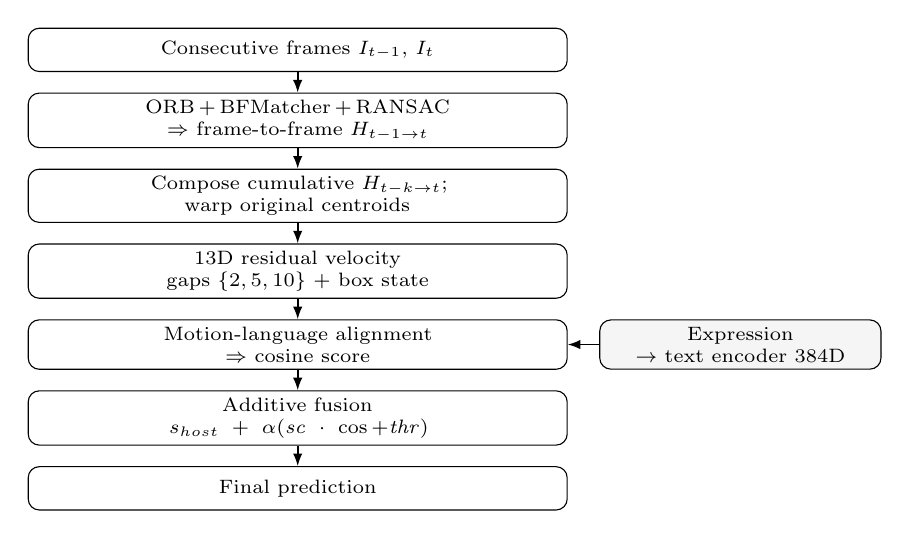
\begin{tikzpicture}[
  font=\scriptsize,
  node distance=2.6mm,
  box/.style={draw, rounded corners, align=center, inner sep=2.5pt,
              text width=0.55\linewidth, minimum height=5.5mm},
  sbox/.style={draw, rounded corners, align=center, inner sep=2.5pt, fill=black!4,
               text width=0.28\linewidth, minimum height=5.5mm},
  ar/.style={-{Latex[length=1.6mm]}, semithick}
]
\node[box] (frames) {Consecutive frames $I_{t-1},\,I_t$};
\node[box, below=of frames] (orb) {ORB\,+\,BFMatcher\,+\,RANSAC\\ $\Rightarrow$ frame-to-frame $H_{t-1\to t}$};
\node[box, below=of orb] (cum) {Compose cumulative $H_{t-k\to t}$;\\ warp original centroids};
\node[box, below=of cum] (desc) {13D residual velocity\\ gaps $\{2,5,10\}$ + box state};
\node[box, below=of desc] (align) {Motion-language alignment\\ $\Rightarrow$ cosine score};
\node[box, below=of align] (fuse) {Additive fusion\\ $s_{\text{host}}+\alpha(\mathit{sc}\cdot\cos+\mathit{thr})$};
\node[box, below=of fuse] (hota) {Final prediction};
\node[sbox, right=4mm of align] (text) {Expression\\ $\to$ text encoder 384D};
\draw[ar] (frames)--(orb);
\draw[ar] (orb)--(cum);
\draw[ar] (cum)--(desc);
\draw[ar] (desc)--(align);
\draw[ar] (align)--(fuse);
\draw[ar] (fuse)--(hota);
\draw[ar] (text)--(align);
\end{tikzpicture}
\caption{\textbf{GMC-Link pipeline.} ORB homographies compose into a cumulative transform, produce a 13D motion feature, align with the expression, and correct the host score through additive fusion.}
\label{fig:pipeline}
\end{figure}

\subsection{Ego-motion compensation}
\label{sec:ego}

This stage estimates camera motion from consecutive video frames so that object motion can be separated from camera-induced motion. Given the input video frames and tracked object bounding boxes, we extract and match background keypoints using ORB~\cite{orb}. Keypoints inside tracked object bounding boxes are removed before matching so that moving foreground objects do not affect camera-motion estimation. The remaining matched keypoints are used with RANSAC~\cite{ransac} to estimate a homography $H_{t-1\to t}$, which describes the geometric transformation caused by camera motion from frame $I_{t-1}$ to frame $I_t$.

To describe camera motion over multiple frames, the estimated homographies are accumulated as
\begin{equation}
H_{t-k\to t} = H_{t-1\to t}\, H_{t-2\to t-1} \cdots H_{t-k\to t-k+1},
\label{eq:cumulative}
\end{equation}
where $H_{t-k\to t}$ represents the accumulated camera transformation from frame $I_{t-k}$ to frame $I_t$. Instead of repeatedly transforming already warped coordinates, the accumulated homography is applied only once to the original object centroid. This reduces numerical drift and provides a stable reference for estimating ego velocity in the next stage.

\subsection{Multi-scale residual velocity}
\label{sec:residual}

Using the accumulated homography from Stage~3.1 together with the tracked object trajectories, this stage estimates residual velocity, which represents object motion after removing the estimated camera motion. For a temporal gap $g$, the raw velocity is the displacement of the object centroid between two frames and therefore contains both object motion and camera-induced motion. The ego velocity is obtained by applying the accumulated homography in Eq.~\ref{eq:cumulative} to the previous object centroid. The residual velocity is computed as
\begin{equation}
v^{\mathrm{res}}_{g} = v^{\mathrm{raw}}_{g} - v^{\mathrm{ego}}_{g},
\label{eq:residual}
\end{equation}
where $v^{\mathrm{res}}_g$, $v^{\mathrm{raw}}_g$, and $v^{\mathrm{ego}}_g$ denote the residual, raw, and ego velocities, respectively. This representation approximates the motion that would be observed by a stationary camera. For example, a parked vehicle has near-zero residual velocity even when camera motion causes a large image displacement. All velocities are normalized by the image dimensions to make them independent of image resolution.

To capture motion over different time spans, residual velocities are computed at temporal gaps of $\{2,5,10\}$ frames. The residual velocities are concatenated with object box information to form a 13-dimensional motion feature,
\begin{equation}
\bigl((dx_s,dy_s),(dx_m,dy_m),(dx_l,dy_l),\Delta w,\Delta h,c_x,c_y,w,h,\rho\bigr),
\label{eq:descriptor}
\end{equation}
where the first six values are the residual velocities at the three temporal gaps and $\Delta w, \Delta h$ capture the change in box scale. The next four values give the box centre and size. The final feature $\rho$ is the ratio between the object's residual speed at the middle gap and the magnitude of the estimated background motion, indicating how far the object's motion stands out from the camera's.

\subsection{Motion-language alignment}
\label{sec:align}

Given the motion feature from Stage~3.2 and the language expression, this stage measures how well the observed object motion matches the described motion. The 13-dimensional motion feature is encoded by a motion encoder, while the language expression is encoded by all-MiniLM-L6-v2 (MiniLM)~\cite{sbert} into a text embedding. Both embeddings are projected into the same feature space using linear projection layers and a shared Multi-Layer Perceptron (MLP).

The model is trained using Information Noise Contrastive Estimation (InfoNCE)~\cite{infonce} loss to maximize the similarity between matched motion-expression pairs while separating unmatched pairs. A positive pair is formed by the motion feature of a tracked object and the expression assigned to that object in the RMOT annotation. Other object--expression pairs in the same mini-batch are treated as negatives. The MiniLM text encoder is kept fixed, and only the projection layers and motion encoder are trained. During inference, the cosine similarity between the motion and language embeddings is used as the motion matching score, which is passed to the decision-level fusion stage described in Section~\ref{sec:fusion}.

\subsection{Decision-level additive fusion}
\label{sec:fusion}

The motion matching score produced in Stage~3.3 is combined with the prediction score of the host RMOT model to obtain the final prediction. The final score is computed as
\begin{equation}
s_{\mathrm{final}} = s_{\mathrm{host}} + \alpha\,\bigl(\mathit{sc}\cdot\cos + \mathit{thr}\bigr),
\label{eq:fusion}
\end{equation}
where $s_{\mathrm{host}}$ is the prediction score produced by the host model, $\cos$ is the cosine similarity from the motion-language alignment stage, $\mathit{sc}$ rescales the motion score to match the score range of the host model, $\mathit{thr}$ adjusts the decision threshold, and $\alpha$ controls the contribution of the motion score.

The calibration parameters are selected once for each host--split setting because different RMOT models produce prediction scores with different ranges. After selection, the coefficients are fixed for all reported experiments and random seeds in that setting. The final coefficients used in this work are listed in Table~\ref{tab:recipe}. During inference, a keyword-based router selects either the motion branch or the appearance branch according to the language expression. Expressions containing motion-related keywords, such as \emph{moving}, \emph{turning}, \emph{parked}, and \emph{braking}, use the motion branch, while all other expressions use the appearance branch.

\begin{table}[t]
\centering
\caption{Locked fusion coefficients for Eq.~\ref{eq:fusion}, selected per host--split setting and then fixed for all reported runs. FlexHook (V1) and (V2) are one architecture calibrated per split. Appearance scale is damped because motion is uninformative on appearance expressions.}
\label{tab:recipe}
\small
\begin{tabular}{llccc}
\toprule
Host & Axis & $\alpha$ & $\mathit{sc}$ & $\mathit{thr}$ \\
\midrule
\multirow{2}{*}{iKUN}        & motion     & 1.00 & 0.90 & $+0.17$ \\
                             & appearance & 1.00 & 0.30 & $+0.10$ \\
\midrule
\multirow{2}{*}{FlexHook (V1)} & motion     & 0.65 & 10.0 & $+3.0$  \\
                             & appearance & 1.00 & 3.50 & $+0.9$  \\
\midrule
\multirow{2}{*}{FlexHook (V2)} & motion     & 0.40 & 10.0 & $+1.3$  \\
                             & appearance & 1.00 & 3.50 & $+1.2$  \\
\bottomrule
\end{tabular}
\end{table}

Since GMC-Link only modifies the final prediction score, it can be integrated into existing two-stage RMOT frameworks without changing or retraining their detector, tracker, visual encoder, or language encoder. The integration is therefore plug-in at the architectural level, but not calibration-free.

\section{Experiments}
\label{sec:exp}

\subsection{Setup}
\label{sec:setup}

We evaluate GMC-Link on the Refer-KITTI V1~\cite{transrmot} and V2~\cite{temprmot} benchmarks using the HOTA metric from TrackEval~\cite{hota}, which jointly measures detection and association performance. Since GMC-Link is designed to improve motion grounding, we report both moving-class HOTA, which evaluates only expressions referring to moving objects, and pooled HOTA, which evaluates all expressions in the benchmark.

To evaluate the effectiveness of GMC-Link under different host capabilities, we attach it to iKUN~\cite{ikun} and FlexHook~\cite{flexhook}. We also compare against a raw-velocity variant that directly uses image-plane motion without ego-motion compensation to measure the contribution of camera motion compensation.

Results are averaged over three random seeds, while ablation studies use five seeds together with Welch's t-test. The reported p-values compare the full GMC-Link module with the raw-velocity variant across the five ablation seeds. The motion-language aligner is trained using AdamW with a learning rate of $10^{-3}$, batch size $256$, and $100$ epochs. Camera motion is estimated using ORB with $1500$ keypoints and RANSAC with a $5$-pixel threshold. Both host models use their original published detection results. For FlexHook V1, our reproduced pipeline remains below the published pooled HOTA; therefore, we report both the difference from the published number and the gain over the reproduced \emph{+GMC simple} anchor.

Refer-KITTI does not provide a dedicated validation split. Therefore, the fusion parameters are calibrated on the benchmark sequences. To evaluate the robustness of this calibration and address possible overfitting, we additionally perform leave-one-sequence-out (LOSO) calibration. In each LOSO run, the parameters are selected using all but one sequence and evaluated on the held-out sequence. Across all evaluated settings, LOSO performance remains above the native host, suggesting that the improvements are not limited to the sequences used for calibration.

Refer-KITTI is highly imbalanced, with only about one-sixth of the language expressions referring to moving objects. Consequently, improvements in motion understanding may have only a limited impact on pooled HOTA. Therefore, moving-class HOTA is used as the primary evaluation metric, while pooled HOTA is reported to reflect overall benchmark performance.

\subsection{Main results}
\label{sec:main}

Table~\ref{tab:main} summarizes the pooled HOTA results on Refer-KITTI. The \emph{+GMC simple} baseline directly adds the motion score without calibration. Its performance is lower than the native host on iKUN and FlexHook V1, showing that simply introducing motion information is not sufficient. The motion score must be calibrated to match the score range of the host model.

After applying the proposed GMC-Link module, performance improves on all settings compared with the uncalibrated baseline. On iKUN, GMC-Link achieves $44.634 \pm 0.066$, which is comparable to the published result ($44.564$) while introducing additional motion reasoning. On FlexHook V2, GMC-Link improves pooled HOTA from $42.526$ to $42.807 \pm 0.038$, showing that the proposed module can also improve pooled performance in this setting. Although FlexHook V1 does not exceed its published score, it outperforms the reproduced uncalibrated baseline, indicating that calibrated motion scores are more effective than directly using raw motion information.

Overall, these results show that camera-motion-compensated motion information is beneficial only when it is properly aligned with the host model. The gains are most visible on motion-referring expressions, while pooled HOTA changes are smaller because motion expressions form a minority of Refer-KITTI. Thus, GMC-Link should be viewed primarily as a motion-grounding correction that preserves competitive pooled performance in the evaluated settings.

\begin{table}[t]
\centering
\caption{Pooled HOTA on Refer-KITTI test ($n{=}3$, mean$\pm$std). $\Delta$ is computed against published pooled HOTA.}
\label{tab:main}
\small
\setlength{\tabcolsep}{4pt}
\begin{tabular}{lcccc}
\toprule
Host & Native & +GMC simple & +GMC-Link & $\Delta$ paper \\
\midrule
iKUN~\cite{ikun} (V1)        & 44.564 & 44.272 & $44.634 \pm 0.066$ & $+0.070$ \\
FlexHook (V1)~\cite{flexhook}  & 53.824 & 53.121 & $53.526 \pm 0.087$ & $-0.298$\textsuperscript{$\dagger$} \\
FlexHook (V2)~\cite{flexhook}  & 42.526 & 42.532 & $42.807 \pm 0.038$ & $+0.281$ \\
\bottomrule
\end{tabular}
\\[2pt]
{\footnotesize \textsuperscript{$\dagger$}FlexHook (V1) paper gap is structural (no tested configuration beats $53.824$); $\Delta$ vs \emph{+GMC simple} anchor $= +0.405$.}
\end{table}

\subsection{Effect on Different Host Models}
\label{sec:deficit}

Table~\ref{tab:deficit} compares the moving-class HOTA improvement across different host models. iKUN, which has the lowest native moving-class HOTA, achieves the largest improvement ($+8.83 \pm 0.83$). In contrast, FlexHook V1 and V2 already have stronger motion reasoning and therefore obtain smaller gains ($+0.91 \pm 0.79$ and $+0.43 \pm 0.17$, respectively).

In our evaluated settings, this trend suggests that GMC-Link is most beneficial for host models with weaker motion understanding. When the host model already distinguishes camera motion from object motion reasonably well, the proposed module provides only a small improvement. Conversely, when the host struggles with motion grounding, GMC-Link can effectively compensate for this limitation and achieve a larger performance gain.

Although this trend is consistent across all evaluated settings, it is observed on two host architectures. Evaluating additional host models would help verify whether this trend generalizes to other architectures.

\begin{table}[t]
\centering
\caption{Effect on different host models. Native moving-class HOTA versus the moving-class HOTA gain added by GMC-Link.}
\label{tab:deficit}
\small
\begin{tabular}{lcc}
\toprule
Host & Native MOVING & GMC MOVING gain \\
\midrule
iKUN~\cite{ikun}             & 20.25 & $+8.83 \pm 0.83$ ($n{=}5$) \\
FlexHook (V1)~\cite{flexhook}  & 43.98 & $+0.91 \pm 0.79$ ($n{=}3$) \\
FlexHook (V2)~\cite{flexhook}  & 48.02 & $+0.43 \pm 0.17$ ($n{=}3$) \\
\bottomrule
\end{tabular}
\\[2pt]
{\footnotesize Moving-class denominators: $27$ of $158$ expressions (V1); $14.2\%$ of $862$ (V2).}
\end{table}

\subsection{Ablations}
\label{sec:ablation}

Table~\ref{tab:ablation} evaluates the contribution of each component in GMC-Link. The full module improves moving-class HOTA from $20.25$ to $29.08$ ($+8.83$). When ego-motion compensation is removed, the score decreases to $27.31$, indicating that simply using image-plane motion already provides useful motion cues, but camera motion compensation is still necessary for the best performance. Compared with this raw-velocity variant, the full module gains $1.77$ moving-class HOTA with Welch's t-test significance ($p{=}0.006$).

Removing ego-motion compensation also reduces static-class HOTA from $43.26$ to $41.19$ ($p{<}10^{-4}$). This is because stationary objects appear to move in the image when the camera moves, causing them to be incorrectly treated as moving objects. In contrast, removing the multi-scale gaps or the residual-to-background ratio $\rho$ produces only small changes that stay within seed variation, suggesting that these components have a relatively limited impact compared with ego-motion compensation.

\begin{table}[t]
\centering
\caption{Per-class HOTA ablation on iKUN ($n{=}5$).}
\label{tab:ablation}
\small
\begin{tabular}{lcc}
\toprule
Variant & MOVING HOTA & STATIC HOTA \\
\midrule
Native host (no module)           & 20.25 & --- \\
Full module                       & \textbf{29.08 $\pm$ 0.83} & \textbf{43.26 $\pm$ 0.26} \\
\;\;$-$ego (raw velocity)         & 27.31 $\pm$ 0.66 & 41.19 $\pm$ 0.39 \\
\;\;$-$multiscale (single gap)    & 28.82 $\pm$ 0.84 & 43.42 $\pm$ 0.10 \\
\;\;$-\rho$ (zeroed slot)         & 29.74 $\pm$ 0.59 & 43.35 $\pm$ 0.35 \\
\bottomrule
\end{tabular}
\\[2pt]
{\footnotesize Native static-class HOTA under the ablation readout is not archived; deltas among module arms share one convention and are directly comparable.}
\end{table}

\begin{figure}[t]
\centering
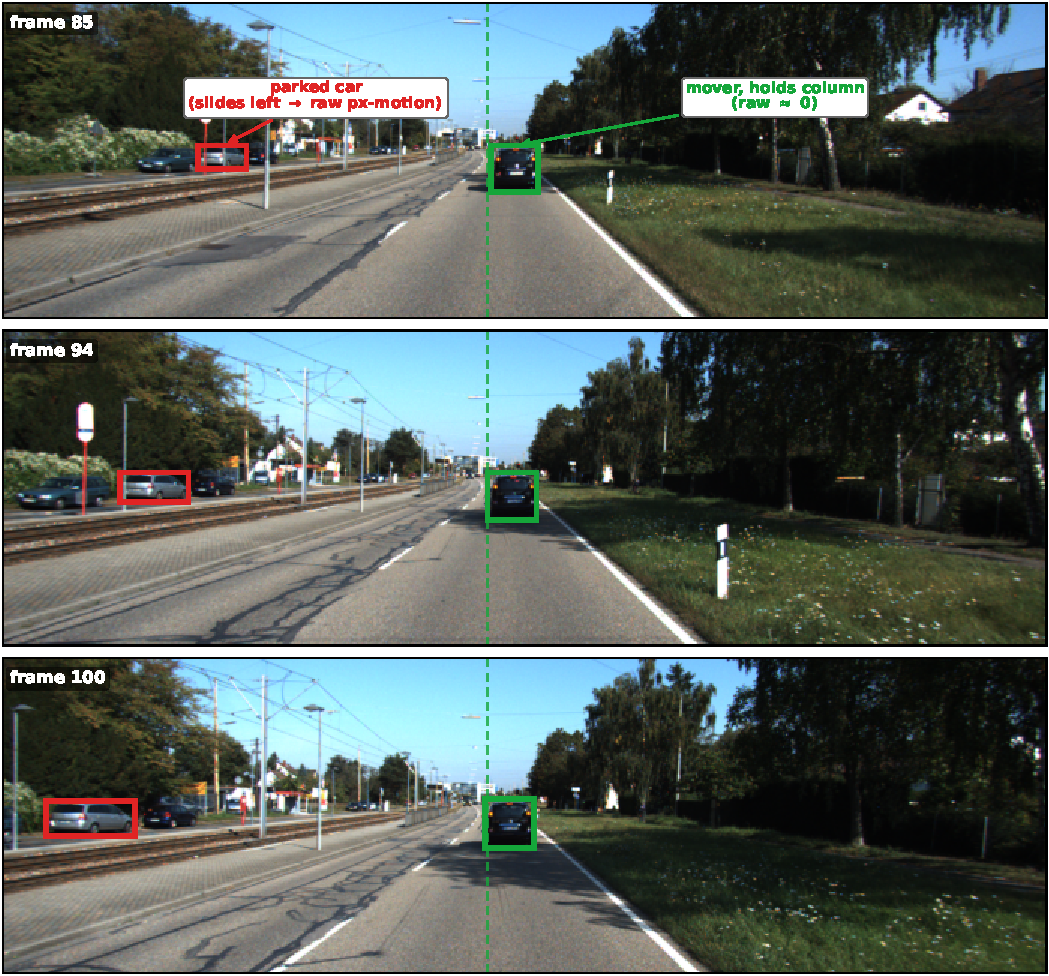
\includegraphics[width=\linewidth]{figures/qualitative.pdf}
\caption{\textbf{Real recovery under camera ego-motion} on ``moving cars'' (Refer-KITTI seq 0005, frames 85/94/100 of a forward-driving clip; the green car moves, the red car is parked). The dashed line marks the mover's image column. \textbf{Red:} the parked car's centroid slides left as the camera passes it (center-$x$ $261\!\to\!104$\,px), so the camera-naive host scores it ``moving'' (false positive), yet its ego-compensated residual is near zero and the module restores it to static. \textbf{Green:} the moving car holds its column (center-$x$ ${\approx}605$, ${<}1$\,px/frame), so the host misses it (false negative), but its nonzero residual --- unlike the static background --- recovers it as moving. Both errors flip from the same host logit through the additive correction.}
\label{fig:qual}
\end{figure}

Figure~\ref{fig:qual} illustrates this behavior using a real example. The parked car moves across the image because of camera motion, while the moving car remains at nearly the same image location. Without ego-motion compensation, these two cases are easily confused because they have similar image-plane motion. After compensating for camera motion, the parked car has nearly zero residual motion, while the moving car retains nonzero residual motion. This allows GMC-Link to correctly distinguish between stationary and moving objects.

Finally, the complete module runs at $68$ FPS (median $14.8$\,ms/frame, excluding host inference), indicating that the proposed module can be integrated into existing RMOT frameworks with low computational overhead.

\section{Conclusion and Limitations}
\label{sec:conclusion}
GMC-Link is a decision-level plug-in module that improves motion grounding in referring multi-object tracking without modifying the detector, tracker, or appearance-language matching model. By compensating for camera motion and aligning residual motion with language descriptions, the proposed module helps distinguish object motion from camera-induced motion. Experimental results on Refer-KITTI show that GMC-Link improves moving-class HOTA in the evaluated host--split settings while maintaining competitive pooled HOTA, suggesting that it can enhance motion understanding without sacrificing overall tracking performance.

Despite these promising results, several limitations remain. First, the proposed camera motion compensation relies on ORB and RANSAC, which estimate a single homography and may become less accurate in scenes with strong parallax or large non-planar motion. Second, the calibration parameters are host-specific and need to be estimated for different host models. Finally, our experiments are conducted on two RMOT frameworks, and additional evaluations on more host architectures and datasets are needed to further validate the generality of the proposed approach.

In future work, we plan to investigate more robust camera motion estimation methods and richer motion features that can better handle complex dynamic scenes. We also hope to evaluate GMC-Link on a broader range of referring multi-object tracking frameworks to further improve its generalization.

\bibliographystyle{ACM-Reference-Format}
\bibliography{refs}

\end{document}
